\documentclass[tikz,border=10pt]{standalone}
\usepackage{amsmath,amssymb}
\usepackage{tikz}
\usetikzlibrary{arrows.meta,positioning,calc,fit,backgrounds,decorations.pathreplacing}

%% ---- Colour palette ----
\definecolor{cBackbone}{RGB}{200,220,245}    % light blue
\definecolor{cBlock}{RGB}{255,230,180}       % light orange
\definecolor{cARR}{RGB}{200,235,200}         % light green
\definecolor{cLoss}{RGB}{250,200,200}        % light red/pink
\definecolor{cHead}{RGB}{230,230,230}        % light gray
\definecolor{cProj}{RGB}{180,210,240}        % medium blue for W_Q/K/V
\definecolor{cDetach}{RGB}{200,80,80}        % red for detach

%% ---- Node styles ----
\tikzset{
  basenode/.style={draw, rounded corners=4pt, minimum height=0.7cm,
                   inner sep=4pt, font=\small\sffamily, align=center},
  backbone/.style={basenode, fill=cBackbone, minimum width=1.8cm},
  block/.style={basenode, fill=cBlock, minimum width=1.5cm},
  arr/.style={basenode, fill=cARR, minimum width=1.8cm},
  loss/.style={basenode, fill=cLoss, minimum width=1.5cm},
  head/.style={basenode, fill=cHead, minimum width=1.5cm},
  proj/.style={basenode, fill=cProj, minimum width=1.0cm, minimum height=0.6cm, font=\footnotesize\sffamily},
  op/.style={basenode, fill=white, minimum width=1.2cm, font=\footnotesize\sffamily},
  arr_op/.style={basenode, fill=cARR!70, minimum width=1.6cm, font=\footnotesize\sffamily},
  myarrow/.style={-{Stealth[length=5pt]}, thick},
  dasharrow/.style={-{Stealth[length=5pt]}, thick, dashed, cDetach},
  labelnode/.style={font=\footnotesize\sffamily, inner sep=1pt},
  groupbox/.style={draw, rounded corners=6pt, thick, inner sep=10pt},
}

\begin{document}
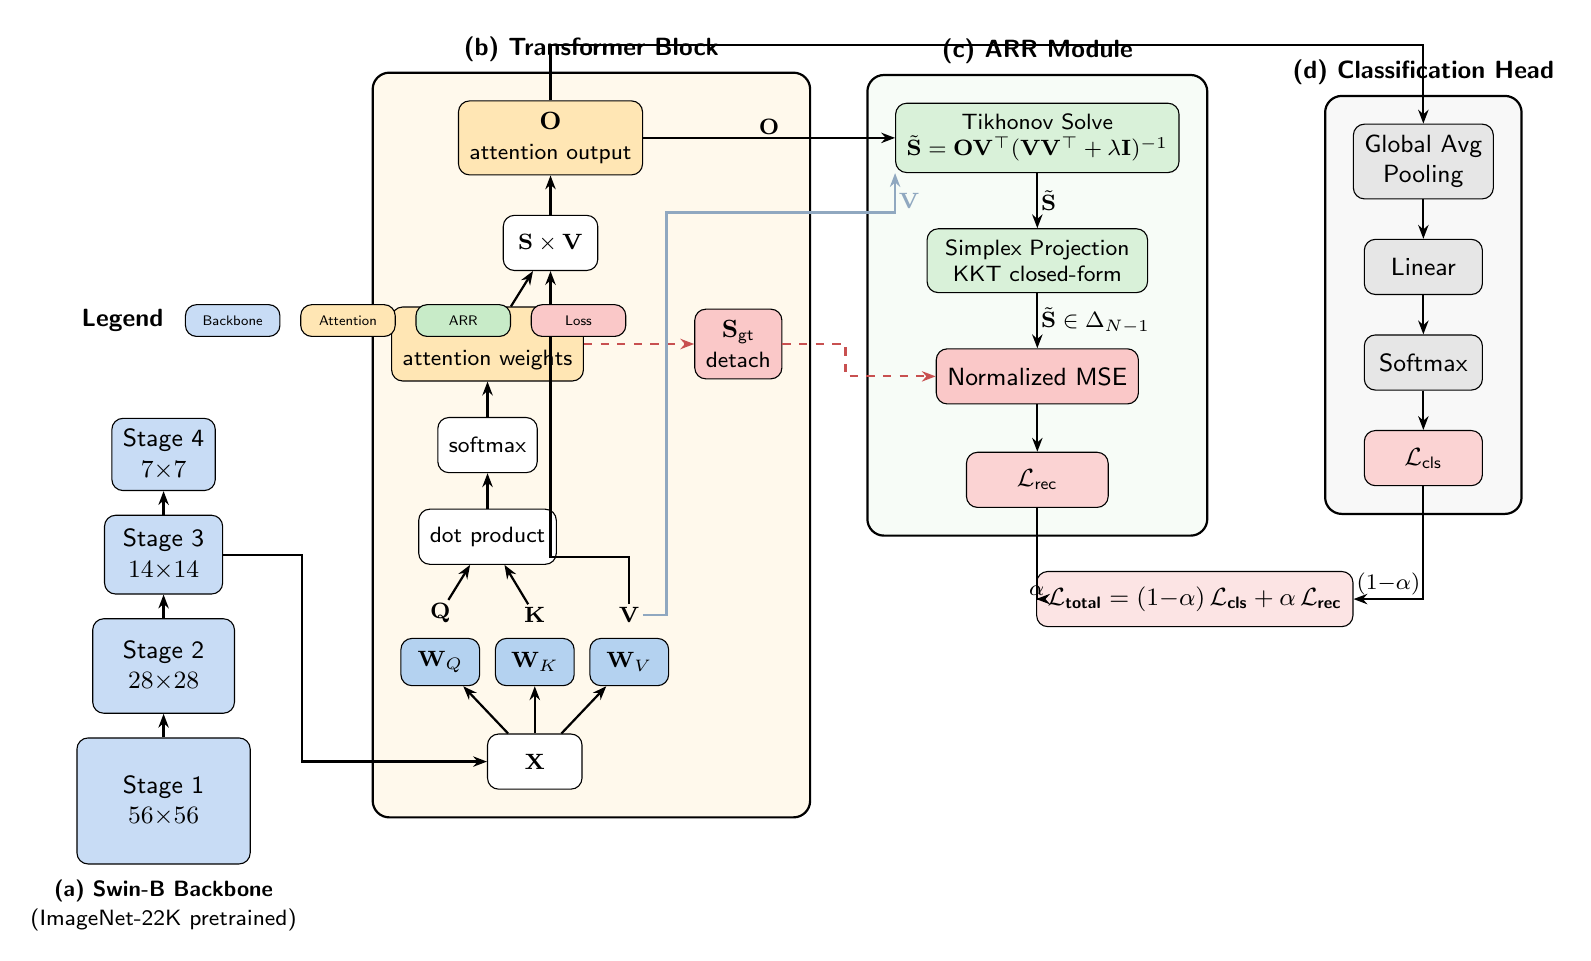
\begin{tikzpicture}[node distance=0.5cm and 0.7cm]

%% ============================================================
%%  (a) Swin-B Backbone (far left column)
%% ============================================================
\node[backbone, minimum height=1.6cm, minimum width=2.2cm] (stage1) {Stage 1\\$56{\times}56$};
\node[backbone, minimum height=1.2cm, minimum width=1.8cm, above=0.3cm of stage1] (stage2) {Stage 2\\$28{\times}28$};
\node[backbone, minimum height=1.0cm, minimum width=1.5cm, above=0.3cm of stage2] (stage3) {Stage 3\\$14{\times}14$};
\node[backbone, minimum height=0.8cm, minimum width=1.2cm, above=0.3cm of stage3] (stage4) {Stage 4\\$7{\times}7$};

\node[labelnode, below=0.15cm of stage1] (bblabel) {\textbf{(a) Swin-B Backbone}};
\node[labelnode, below=0.0cm of bblabel] {(ImageNet-22K pretrained)};

\draw[myarrow] (stage1) -- (stage2);
\draw[myarrow] (stage2) -- (stage3);
\draw[myarrow] (stage3) -- (stage4);

%% ============================================================
%%  (b) Transformer Block Detail
%%  X -> W_Q/W_K/W_V -> dot product / V -> softmax -> S -> SxV -> O
%%  S_gt detached from S
%% ============================================================
\node[op, right=3.0cm of stage1, yshift=0.5cm] (inputX) {$\mathbf{X}$};

%% W_Q, W_K, W_V projections
\node[proj, above=0.6cm of inputX, xshift=-1.2cm] (WQ) {$\mathbf{W}_Q$};
\node[proj, above=0.6cm of inputX] (WK) {$\mathbf{W}_K$};
\node[proj, above=0.6cm of inputX, xshift=1.2cm] (WV) {$\mathbf{W}_V$};

\draw[myarrow] (inputX) -- (WQ);
\draw[myarrow] (inputX) -- (WK);
\draw[myarrow] (inputX) -- (WV);

%% Q, K, V labels
\node[labelnode, above=0.15cm of WQ] (Q) {$\mathbf{Q}$};
\node[labelnode, above=0.15cm of WK] (K) {$\mathbf{K}$};
\node[labelnode, above=0.15cm of WV] (V) {$\mathbf{V}$};

%% dot product -- Q and K
\node[op, above=0.5cm of K, xshift=-0.6cm] (dot) {dot product};
\draw[myarrow] (Q) -- (dot);
\draw[myarrow] (K) -- (dot);

%% softmax
\node[op, above=0.45cm of dot] (softmax) {softmax};
\draw[myarrow] (dot) -- (softmax);

%% S (attention weights)
\node[block, above=0.45cm of softmax, minimum width=1.8cm] (S) {$\mathbf{S}$\\{\footnotesize attention weights}};
\draw[myarrow] (softmax) -- (S);

%% S x V
\node[op, above=0.45cm of S, xshift=0.8cm] (SV) {$\mathbf{S} \times \mathbf{V}$};
\draw[myarrow] (S) -- (SV);
%% V -> SV: go up along right side, clean L-shaped path
\draw[myarrow] (V.north) -- ++(0,0.6) -| (SV.south);

%% O (output)
\node[block, above=0.5cm of SV, minimum width=2.0cm] (O) {$\mathbf{O}$\\{\footnotesize attention output}};
\draw[myarrow] (SV) -- (O);

%% S_gt (detached) -- placed to the right of S
\node[loss, right=1.4cm of S, minimum width=1.0cm] (Sgt) {$\mathbf{S}_{\text{gt}}$\\{\footnotesize detach}};
\draw[dasharrow] (S.east) -- (Sgt.west);

%% group box for transformer block
\begin{scope}[on background layer]
  \node[groupbox, fill=cBlock!25, fit=(inputX)(WQ)(WV)(O)(Sgt),
        label={[font=\small\sffamily\bfseries]above:\textbf{(b) Transformer Block}}] (blockbox) {};
\end{scope}

%% arrow from backbone Stage 3 to block input X
\draw[myarrow, thick] (stage3.east) -- ++(1.0,0) |- (inputX.west);

%% ============================================================
%%  (c) ARR Module
%%  Vertical top-to-bottom: Tikhonov -> Simplex -> NormMSE -> L_rec
%%  Inputs: O (from top-left), V (from left), S_gt (from left)
%% ============================================================

%% Place Tikhonov to the right of O, with generous spacing
\node[arr_op, right=3.2cm of O, minimum width=3.2cm] (tikhonov)
  {Tikhonov Solve\\$\tilde{\mathbf{S}} = \mathbf{O}\mathbf{V}^\top(\mathbf{V}\mathbf{V}^\top + \lambda\mathbf{I})^{-1}$};

%% O -> Tikhonov: straight horizontal, top connection
\draw[myarrow] (O.east) -- node[above, labelnode] {$\mathbf{O}$} (tikhonov.west);

%% Simplex Projection
\node[arr_op, below=0.7cm of tikhonov, minimum width=2.8cm] (simplex)
  {Simplex Projection\\{\footnotesize KKT closed-form}};
\draw[myarrow] (tikhonov) -- node[right, labelnode] {$\tilde{\mathbf{S}}$} (simplex);

%% Normalized MSE
\node[loss, below=0.7cm of simplex, minimum width=2.4cm] (nmse) {Normalized MSE};
\draw[myarrow] (simplex) -- node[right, labelnode] {$\tilde{\mathbf{S}} \in \Delta_{N-1}$} (nmse);

%% L_rec
\node[loss, below=0.6cm of nmse, minimum width=1.8cm, fill=cLoss!80] (Lrec) {$\mathcal{L}_{\text{rec}}$};
\draw[myarrow] (nmse) -- (Lrec);

%% V -> Tikhonov: from V label, go right then up, enter Tikhonov from below-left
\draw[myarrow, cProj!80!black]
  (V.east) -- ++(0.3,0)                              % short stub right from V label
  |- ([yshift=-0.5cm]tikhonov.south west)             % go up to below Tikhonov
  -- ([yshift=0cm]tikhonov.south west)                % enter from bottom-left corner area
  node[pos=0.0, above right, labelnode] {$\mathbf{V}$};

%% S_gt -> Normalized MSE: route right from S_gt then down, entering nmse from left
%% This avoids crossing the vertical Tikhonov->Simplex->NormMSE chain
\draw[dasharrow]
  (Sgt.east) -- ++(0.8,0)    % go right
  |- (nmse.west);             % then down and into nmse from the left

%% group box for ARR
\begin{scope}[on background layer]
  \node[groupbox, fill=cARR!15, fit=(tikhonov)(simplex)(nmse)(Lrec),
        label={[font=\small\sffamily\bfseries]above:\textbf{(c) ARR Module}}] (arrbox) {};
\end{scope}

%% ============================================================
%%  (d) Classification Head (far right)
%% ============================================================
\node[head, right=2.2cm of tikhonov, yshift=-0.3cm] (gap) {Global Avg\\Pooling};
\node[head, below=0.5cm of gap] (linear) {Linear};
\node[head, below=0.5cm of linear] (softmax2) {Softmax};
\node[loss, below=0.5cm of softmax2, minimum width=1.5cm, fill=cLoss!80] (Lcls) {$\mathcal{L}_{\text{cls}}$};

\draw[myarrow] (gap) -- (linear);
\draw[myarrow] (linear) -- (softmax2);
\draw[myarrow] (softmax2) -- (Lcls);

%% O -> Classification Head: route above everything, no crossing
\draw[myarrow] (O.north) -- ++(0,0.7) -| (gap.north);

%% group box for classification head
\begin{scope}[on background layer]
  \node[groupbox, fill=cHead!30, fit=(gap)(linear)(softmax2)(Lcls),
        label={[font=\small\sffamily\bfseries]above:\textbf{(d) Classification Head}}] (headbox) {};
\end{scope}

%% ============================================================
%%  Loss combination (bottom, between ARR and Head)
%% ============================================================
\node[loss, below=0.8cm of Lrec, xshift=2.0cm, minimum width=3.8cm,
      fill=cLoss!50, font=\small\sffamily\bfseries]
  (Ltotal) {$\mathcal{L}_{\text{total}} = (1{-}\alpha)\,\mathcal{L}_{\text{cls}} + \alpha\,\mathcal{L}_{\text{rec}}$};

\draw[myarrow] (Lrec.south) |- (Ltotal.west)
  node[pos=0.75, above, labelnode] {$\alpha$};
\draw[myarrow] (Lcls.south) |- (Ltotal.east)
  node[pos=0.75, above, labelnode] {$(1{-}\alpha)$};

%% ============================================================
%%  Legend (top left)
%% ============================================================
\node[anchor=north west, font=\small\sffamily\bfseries] at ($(stage4.north west)+(-0.5,1.5)$) (legendtitle) {Legend};
\node[backbone, minimum width=1.2cm, minimum height=0.4cm, right=0.15cm of legendtitle, anchor=west, font=\tiny\sffamily] (leg1) {Backbone};
\node[block, minimum width=1.2cm, minimum height=0.4cm, right=0.25cm of leg1, anchor=west, font=\tiny\sffamily] (leg2) {Attention};
\node[arr, minimum width=1.2cm, minimum height=0.4cm, right=0.25cm of leg2, anchor=west, font=\tiny\sffamily] (leg3) {ARR};
\node[loss, minimum width=1.2cm, minimum height=0.4cm, right=0.25cm of leg3, anchor=west, font=\tiny\sffamily] (leg4) {Loss};

\end{tikzpicture}
\end{document}
